
\section{The Apriori Algorithm \inv}

Previous work on database-centric data mining applications has shown
that these are not supported well by current O-R systems, and there is
no clear understanding on which SQL extensions are needed to solve the
problem. In elucidating this sorry state of affairs the award winning
paper~\cite{cachemine} also established the Apriori algorithm as the
litmus test that any aspiring solution must satisfy.  The AXL
system~\cite{vldb2k} failed this acid test---also all the applications
presented in Section 4 and some of those discussed in Section 3 could
not be supported in AXL. These setbacks helped us identifying
important features that were missing from AXL and various aspects of
its implementation architecture and query optimizer that required
major improvements.  The new features added to ATLaS include support
for (i) table functions coded in SQL, (ii) in-memory tables, (iii)
OIDs used to reference tuples and implement (in-memory) data
structures, and (iv) many changes in the optimizer to improve the
execution speed of programs.
%the trie data structure used in the Apriori algorithm.
These improvements have produced the ATLaS system that supports
efficiently a wide spectrum of data-intensive applications, including
the Apriori algorithm.


\paragraph{Problem Statement.} The problem of mining frequent itemsets over
basket data was introduced by R. Agrawal et al. in~\cite{agg94}.
%An example of such rules
%might be that 98\% of customers that purchase tires and auto
%accessories also get automotive services done.
% Finding all such rules is valuable
% for cross-marketing and attached mailing applications.
Let $I=\{i_1, ..., i_m\}$ be a set of literals, called items. Let $D$
be a set of transactions, where each transaction $T$ is a set of
items.  We say that a transaction $T$ contains itemset $X$, if
$T\supseteq X$. Itemset $X$ has support $s$ in the transaction set $D$
if no less than $s$ transactions in $D$ contain $X$.
Given a set of transactions $D$, the problem of mining frequent
itemsets is to generate all itemsets that have support greater than
the user-specified minimum support (called $MinSup$).

\paragraph{Data Organization.} Let a transaction dataset be represented by
a stream of items, and each item is encoded with an integer $t$,
$t>0$. Adjacent transactions in the stream are separated by a special
symbol, 0.  Within each transaction, items are sorted by their integer
value. For example, the following stream represents a dataset of 5
transactions:
\begin{equation}
{\bf 0},2,3,4,{\bf 0},1,2,3,4,{\bf 0},3,4,5,{\bf 0},1,2,5,{\bf 0},2,4,5
\label{equ:data}
\end{equation}
Thus, we assume that this stream is drawn from a database table:
{\bw baskets(item} {\cw INT)}.

However, our algorithm does not depend on the existence of such a
table, since it will work for data taken from a stream, a view, or
generated by a query.

We use a prefix tree, or a trie, to store frequent itemsets. An
example trie is shown in Figure~\ref{fig:trie:a}. Each node in the
trie represents a frequent itemset that contains all the items on the
path from the root to that node. For instance, the only frequent
3-itemset in Figure~\ref{fig:trie:a} is (2,3,4). In ATLaS, the trie is
represented by the in-memory table {\bw trie}, where each
record contains an item, as well as a pointer to its parent node,
which is another record in the {\bw trie} table:
{\cw  \ \ {\bw trie(itno} INT, {\bw father} REF{\bw (trie)}).}

The trie grows level-by-level. To find frequent $(k+1)$-itemsets, we
first generate candidates based on the $k$-itemsets. The candidates
are stored in an in-memory table: {\cw {\bw cands}({\bw cit} Int, {\bw
    trieref } REF{\bw(trie), freqcount} {\cw Int)}.}


Each record in {\bw cands} contains an item, {\bw cit}, and a
reference, {\bw trieref}, which points to a leaf node of the trie.  If
the leaf node is on level $k$, then {\bw cit}, together with the
frequent itemset referenced by {\bw trieref}, represents a candidate
itemset of $k+1$ items. The support of the candidate, {\bw freqcount},
is updated in the algorithm as we count its occurrence.
For efficiency purposes, both {\bw trie} and {\bw cands} are indexed.
More specifically, {\bw trie} is indexed on {\bw father},
and {\bw cands} is indexed on the pair {\bw (cit,trieref)}.

{\renewcommand{\baselinestretch}{1}
\normalsize

\begin{algorithm}[tb]
%\begin{algorithm}[!htb]
\begin{algorithmic}[1]

  \STATE\kw{TABLE} baskets(item \kw{Int}) \kw{SOURCE}(marketdata);\\
  \STATE\kw{TABLE} trie(item \kw{Int}, father \kw{REF}(trie)) \kw{INDEX}(father) \kw{MEMORY};\\
  \STATE\kw{TABLE} cands(item \kw{Int}, trieref \kw{REF}(trie), freqcount \kw{Int})
   \kw{INDEX}(cit,trieref) \kw{MEMORY};\\
  \STATE\kw{TABLE} fitems(item \kw{Int}) \kw{INDEX}(item);\\
  \COMMENT{generat frequent one-itemsets}
  \STATE\kw{INSERT INTO} fitems \\
  \hspace{.4cm}\kw{SELECT} item \kw{FROM} baskets \kw{WHERE} item $>$ 0 \\
  \hspace{.4cm}\kw{GROUP BY} item \kw{HAVING} count(*) $\ge MinSup$;\\
  \COMMENT{intialize the trie to contain frequent one-itemsets}
  \STATE\kw{INSERT} \kw{INTO} trie \kw{SELECT} item, null \kw{FROM} fitems;\\
  \COMMENT{self-join frequent 1-itemsets to get candidate 2-itemsets}
  \STATE\kw{INSERT} \kw{INTO} cands \kw{SELECT} t1.itno, t2.OID, 0 \kw{FROM} trie \kw{AS} t1, trie \kw{AS} t2 \alglabel{algwhere} \kw{WHERE} t1.itno $>$ t2.itno;\\
  \COMMENT{Generate (k+1)-itemsets from k-itemsets. Start with
    k=2}
  \STATE\kw{SELECT} countset(item, 2, $MinSup$, cands) \kw{FROM} baskets;
\end{algorithmic}
\caption{Main ATLaS Program for Apriori}
\label{alg:apriori}
\end{algorithm}

\inv \paragraph{The Algorithm.} The ATLaS implementation of Apriori is shown in
Algorithm~\ref{alg:apriori}.  First, we scan the dataset to find out
frequent 1-itemsets and insert them into the trie. Next, we self-join
the frequent 1-itemsets to generate candidate 2-itemsets. The {\cw
  WHERE} condition on line~\algref{algwhere} guarantees that each
frequent itemset is uniquely represented in the trie --- a child node
is always labelled with a larger item than its parent.  After the join
operation (assuming we are mining the sample dataset in (\ref{equ:data}) with a
threshold $MinSup=2$), the contents of table {\bw trie} and {\bw cand}
can be depicted by Figure~\ref{fig:trie:b}. Finally, we invoke UDA
{\bw countset} to extend the trie to higher levels.

The implementation of {\bw countset} is shown in
Algorithm~\ref{alg:countset}, which recursively extends the trie
level-by-level until no more frequent itemsets can be found.

\begin{figure}[htb]
\subfigure[Trie: each node represents a frequent itemset]{
\label{fig:trie:a}
\begin{minipage}[b]{.5\textwidth}
\centering
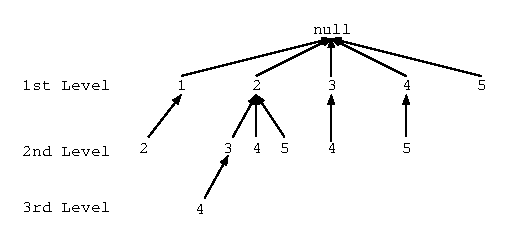
\includegraphics[height=2.5cm,width=7cm]{triefinal.eps}
\end{minipage}
}
\subfigure[Trie and candidate itemsets on the 2nd-level]{
\label{fig:trie:b}
\begin{minipage}[b]{.5\textwidth}
\centering
\includegraphics[height=2.5cm,width=7cm]{trie.eps}
\end{minipage}
}
\caption{Representing the trie in a relational table with the reference data type}
\end{figure}

{\renewcommand{\baselinestretch}{1}
\normalsize

\begin{algorithm}[!htb]
\begin{algorithmic}[1]

\STATE\kw{AGGREGATE} countset (bitem \kw{Int}, J \kw{Int}, $MinSup$ \kw{Int}, cands \kw{TABLE})\\
\STATE\{\hspace{.1cm}\kw{TABLE} previous(marked \kw{REF}(trie), Level \kw{Int})
 \kw{INDEX}(marked) \kw{MEMORY}; \\
\STATE\hspace{.3cm}\kw{TABLE} nextcands(cit \kw{Int}, trieref \kw{REF}(trie),
freqcount \kw{Int}) \kw{INDEX}(trieref) \kw{MEMORY};\\

\STATE\hspace{.3cm}\kw{INITIALIZE}: \kw{ITERATE}: \{ \\
\hspace{.6cm}\COMMENT{Intialize previous for a new transaction if bitem=0.}
\STATE\hspace{.6cm}\kw{DELETE} \kw{FROM} previous \kw{WHERE} bitem=0;\\
\STATE\hspace{.6cm}\kw{INSERT} \kw{INTO} previous \kw{VALUES} (null, 0) \kw{WHERE} bitem=0;\\
\hspace{.6cm}\COMMENT{Store supported frequent itemsets in previous}
\STATE\alglabel{algprev}\hspace{.6cm}\kw{INSERT} \kw{INTO} previous\\
\hspace{.9cm}\kw{SELECT} t.OID, p.Level+1 \kw{FROM} previous \kw{AS} p, trie \kw{AS} t\\
\hspace{.9cm}\kw{WHERE} t.itno=bitem \kw{AND} t.father=p.marked \kw{AND} p.Level$<$J-1;\\
\hspace{.6cm}\COMMENT{Count candidates that appear in the transaction}
\STATE\alglabel{algaddcount}\hspace{.6cm}\kw{UPDATE} cands \kw{SET} freqcount=freqcount+1 \\
\hspace{.9cm}\kw{WHERE} bitem $>$ 0 \kw{AND} c.cit=bitem\\
\hspace{1.3cm}\kw{AND} OID = (\kw{SELECT} c.OID \kw{FROM} previous \kw{AS} p, cands \kw{AS} c\\
\hspace{3.3cm}\kw{WHERE} p.Level=J-1 \kw{AND} c.trieref=p.marked);\\
\STATE\hspace{.2cm}\}\\

\STATE\hspace{.2cm}\kw{TERMINATE}: \{\hspace{.5cm}\\
% \STATE\hspace{1cm}\kw{DELETE} \kw{FROM} cands \kw{WHERE} freqcount $< MinSup$;\\
% \STATE\hspace{1cm}\kw{INSERT INTO} trie \kw{SELECT} cit,trieref \kw{FROM} cands;\\
\hspace{.6cm}\COMMENT{Derive  trie on level J and candidates on level J+1}
\STATE\alglabel{alggrow}\hspace{.6cm}\kw{INSERT} \kw{INTO} nextcands\\
\hspace{.9cm}\kw{SELECT} nextlevel (cit, trieref) \kw{FROM} cands \kw{WHERE} freqcount $\ge MinSup$ \kw{GROUP BY} trieref;\\
% \STATE\hspace{1cm}\kw{DELETE} \kw{FROM} cands;\\
% \STATE\hspace{1cm}\kw{INSERT} \kw{INTO} cands \kw{SELECT} * \kw{FROM} nextcands;\\
\hspace{.6cm}\COMMENT{Eliminate candidates by the anti-monotonicity}
\STATE\alglabel{alganti}\hspace{.6cm}\kw{INSERT} \kw{INTO} subitems \kw{VALUES}(null,0);\\
\STATE\hspace{.6cm}\kw{SELECT} checkset(cit, trieref), antimon(cit, trieref, J) \kw{FROM} nextcands; \\
\hspace{.6cm}\COMMENT{Ascend to level J+1 if cands not empty}
\STATE\alglabel{algrec}\hspace{.6cm}\kw{SELECT} countset (b.item, J+1, $MinSup$, nextcands) \\
\hspace{.9cm}\kw{FROM} (\kw{SELECT} count(*) \kw{AS} size \kw{FROM} nextcands) \kw{AS} c, baskets \kw{AS} b \kw{WHERE} c.size $>$0;\\
\hspace{.3cm}\}\\
\STATE\}
\end{algorithmic}
\caption{countset}
\label{alg:countset}
\end{algorithm}
The {\cw INITIALIZE} and {\cw ITERATE} routine of UDA {\bw countset}
is responsible for counting the occurrences of each candidate. As we
scan through each item in a transaction, we traverse the trie and
incrementally find all the itemsets that are supported by the
transaction, and we store the references to these itemsets in the {\bw
  previous} table (line~\algref{algprev}), which is initialized to
contain nothing but the root node at the beginning of each
transaction. On line~\algref{algaddcount}, the count of the candidate
is increased by 1 if the candidate itemset is supported by the
transaction. We will now continue with our example starting from the
trie in Figure~\ref{fig:trie:b}: after the first transaction,
$(2,3,4)$, is processed by {\bw countset}, table {\bw previous}
contains 4 nodes, namely the root, and nodes $2,3$, and $4$; also,
three candidate itemsets, $(2,3), (2,4)$, and $(3,4)$, have their
counts updated.

The {\cw TERMINATE} routine of {\bw countset} is responsible for
extending the trie to a new level.  On line~\algref{alggrow}, we call
{\bw nextlevel} to extend the trie to level $J$ by adding
candidates with a support no less than $MinSup$ to the trie.  The UDA {\bw
  nextlevel} also generates candidates on level $J+1$. Then, we apply
the anti-monotonic property to filter the candidates. This is
achieved by calling  {\bw checkset} and {\bw antimon} on
line~\algref{alganti}. Finally, on line~\algref{algrec}, we
recursively invoke {\bw countset} to extend the trie to level $J+1$
unless no new candidates are found.

{\renewcommand{\baselinestretch}{1}
\normalsize

\begin{algorithm}[!htb]
\begin{algorithmic}[1]
  \STATE\kw{TABLE} subitems(toid \kw{REF}(trie), level \kw{Int}) \kw{MEMORY};\\
  \COMMENT{extend the trie and return candidates on the new level}\\
  \STATE\kw{AGGREGATE} nextlevel(item \kw{Int}, ptrie \kw{REF}(trie)): (\kw{Int}, \kw{REF}(trie), \kw{Int})\\
  \STATE\{\hspace{.1cm}\kw{TABLE} previous(poid \kw{REF}(trie)) \kw{MEMORY};\\
  \STATE\hspace{.3cm}\kw{INITIALIZE}: \kw{ITERATE}: \{\\
  \STATE\alglabel{algext}\hspace{.6cm}\kw{INSERT} \kw{INTO} trie \kw{VALUES}(item, ptrie);\\
  \hspace{.6cm}\COMMENT{join with previously inserted itemsets and return them as next-level candidates}\\
  \STATE\hspace{.6cm}\kw{INSERT} \kw{INTO} \kw{RETURN} \kw{SELECT} item, previous.poid, 0 \kw{FROM} previous;\\
  \hspace{.6cm}\COMMENT{appending the newly-added to the previous
    table}
  \STATE\hspace{.6cm}\kw{INSERT} \kw{INTO} previous \\
  \hspace{.9cm}\kw{SELECT} trie.OID \kw{FROM} trie \kw{WHERE} trie.itno=item \kw{AND} trie.father=ptrie;\\
  \hspace{.3cm}\}\\
  \STATE\}\\
  \COMMENT{for each (J+1)-itemset, find its frequent subsets of size J}\\
  \STATE\kw{AGGREGATE} checkset (citem \kw{Int}, cref \kw{REF}(trie))\\
  \STATE\{\hspace{.2cm}\kw{INITIALIZE}: \kw{ITERATE}: \{\hspace{.5cm}\\
  \hspace{.6cm}\COMMENT {call checkset recursively}\\
  \STATE\hspace{.6cm}\kw{SELECT} checkset(f.itno, f.father) \kw{FROM} trie \kw{AS} f \kw{WHERE} cref$<>$null \kw{AND} f.OID=cref;\\
  \hspace{.6cm}\COMMENT {as we exit the recursion we expand subitems}\\
  \STATE\hspace{.6cm}\kw{INSERT} \kw{INTO} subitems \\
  \hspace{.9cm}\kw{SELECT} t.OID, s.level+1 \kw{FROM} subitems \kw{AS} s, trie \kw{AS} t\\
  \hspace{.9cm}\kw{WHERE} t.itno=citem \kw{AND} t.father=s.toid;\\
  \hspace{.3cm}\}\\
  \STATE\}\\
  \COMMENT{pruning using the anti-monotonic property}\\
  \STATE\kw{AGGREGATE} antimon(it \kw{Int}, aref \kw{REF}(trie), J \kw{Int})\\
  \STATE\{\hspace{.1cm}\kw{INITIALIZE}: \kw{ITERATE}: \{ \\
%  \hspace{.6cm}\COMMENT{eliminating a candidate if it has at least one subset of size J that is not frequent}\\
  \STATE\hspace{.6cm}\kw{DELETE} \kw{FROM} cands \\
  \hspace{.9cm}\kw{WHERE} cands.cit=it \kw{AND} trieref=aref\\
  \hspace{1.3cm}\kw{AND} J+1 $>$ (\kw{SELECT} count(*) \kw{FROM} subitems \kw{WHERE} subitems.level=J);\\
%  \hspace{.6cm}\COMMENT{reset the subitems table}\\
  \STATE\hspace{.6cm}\kw{DELETE} \kw{FROM} subitems \kw{WHERE} toid $<>$ null;\\
  \hspace{.2cm}\}
  \STATE\}
\end{algorithmic}
\caption{Supporting UDAs for Apriori}
\label{alg:support}
\end{algorithm}


\begin{figure}[htb!]
\subfigure[After invoking UDA {\bw nextlevel}]{
\label{fig:trie:c}
\begin{minipage}[b]{.5\textwidth}
\centering
\includegraphics[height=2.5cm,width=7cm]{trieprune.eps}
\end{minipage}
}
\subfigure[After invoking UDA {\bw checkset} and {\bw antimon}]{
\label{fig:trie:d}
\begin{minipage}[b]{.5\textwidth}
\centering
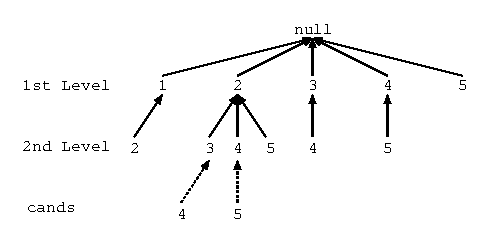
\includegraphics[height=2.5cm,width=7cm]{trieanti.eps}
\end{minipage}
}
\caption{Candidates generation and pruning}
\end{figure}

The UDA {\bw nextlevel} adds each qualified candidate onto the trie
(line~\algref{algext} in Algorithm~\ref{alg:support}).  It also
generates the next-level candidates by computing the self-join of the
newly added itemsets; this UDA is called with a {\cw GROUP BY} clause
to exclude candidates that do not share the same parent\footnote{A
  candidate resulting from self-joining itemsets that do not share the
  same parent is already included in the join result of
  itemsets that share the same parent, or will be eliminated by the
  anti-monotonic property.}.  The join operation is carried out
through the use of a temporary table called {\bw previous}, which
stores all the itemsets that appear ahead of the current itemset, and
they are joined with the current itemset to generate candidates on the
new level.  Figure~\ref{fig:trie:c} shows the result after {\bw
  nextlevel} is applied: qualified candidates in
Figure~\ref{fig:trie:b} become a new level of nodes in the trie, and a
new set of candidates are derived by self-joining the itemsets on
Level 2.

UDA {\bw checkset} and {\bw antimon} together implement the
anti-monotonic property for pruning. For each candidate itemset on
level $J+1$, {\bw checkset} traverses the trie to find all of its
sub-itemsets. According to the anti-monotonic property, a necessary
condition for a $(J+1)$-itemset to be a frequent itemset is that each
of its $J+1$ subsets is a frequent itemset. Thus, {\bw antimon}
eliminates those candidates that have fewer than $J+1$ frequent
itemsets of size $J$.  Figure~\ref{fig:trie:d} shows the result after
{\bw antimon} has eliminated candidate $(2,3,5)$ from
Figure~\ref{fig:trie:c}: $(2,3,5)$ cannot be a frequent itemset
because one of its subset, $(3,5)$, is not frequent.

As shown in Figure~\ref{fig:trie:a}, the
process on the sample dataset terminates at level 3.  At that point,
table {\bw trie} contain all the results, i.e., the frequent itemsets. \inv
